\documentclass[a4paper]{report} 
\usepackage{listings}
\usepackage{amsmath,amssymb}
\usepackage{tikz}
\renewcommand{\thesection}{\arabic{section}}
\renewcommand{\thesubsection}{\thesection.\alph{subsection}}
\title{Tema 1 Algoritmi Avansati}
\author{Sociu Daniel}
\begin{document}

\chapter*{TSP}
\addcontentsline{toc}{chapter}{TSP}
\setcounter{section}{0}
\section{Problema 1}
TSP unde muchiile au ponderea 1 sau 2. 

Sa pp. ca $\exists$ un algoritm polinomial si aproximativ $ALG\leq cOPT$ unde OPT e o rezolvare optima pentru TSP.

\subsection{}

Fie $G$ graful cu n noduri si ponderi 1 si 2 $\rightarrow$ observam ca $OPT$ e maxim $2n$.

Stim ca problema determinarii unui HC in G este NPC.

Construim $G'$ complet, muchiile comune intre $G$ si $G'$ isi pastreaza costul iar celelalte muchii vor avea costul $c\cdot 2n$. Acum avem 2 cazuri:

\begin{enumerate}
    \item daca G are un HC $\implies ALG$ va oferi un traseu de cost cel mult $c\cdot 2n$
    \item daca G nu are un HC $\implies ALG$ va oferi cel mai bun traseu posibil cu cel mult $n-1$ noduri de cost 1 si 2, iar restul de cost $c\cdot 2n$.
        Adica cel mai bun traseu va fi $ALG \geq (n-1) + c\cdot 2n$
\end{enumerate}

Adica putem determina in timp polinomial daca $G$ este sau nu Hamiltonian $\implies$ HC se poate rezolva in timp polinomial. Contradictie (HC e NPC)!\\

Deci aceasta varianta a TSP-ului este tot NP-hard.

\subsection{}

Regula triunghiului $L_{3}\geq L_{2} \geq L_{1} \implies L_{3}\leq L_{2} + L_{1}$

Deci pentru a demonstra ca regula triunghiului tine trebuie sa selectam $L_{3}$ maximul posibil si elementele $L_{2}$ si $L_{1}$ minime

Adica vom considera $L_{3}=2$ si $L_{2}=1, L_{1}=1$ $\implies 2\leq 1 \leq 1$ si $2\leq 1 + 1$ adevarate deci regula triunghiului tine in aceasta instanta. 

\subsection{}

Am vazut din curs ca daca $len((u,v))\leq len((u,w)) + len((w,v))$ atunci si relatia urmatoare are loc:
\[len((v_{1},v_{k}))\leq len(v_{1},v_{2} \dots v_{k}) \text{ unde } v_{1},v_{2} \dots v_{k} \text{ e un lant.}\]

Mai stim din curs ca $OPT\geq MST$\\

Considerand acelasi algoritm descris in curs, care se bazeaza pe un MST, sa presupunem ca avem $ALG\leq \frac{3}{2}MST \leq\frac{3}{2}OPT$. Observam ca din cauza ca $MST$
e un lower bound pentru $OPT$ trebuie sa aratam direct ca $ALG> \frac{3}{2}OPT$

Fie graful G:\\

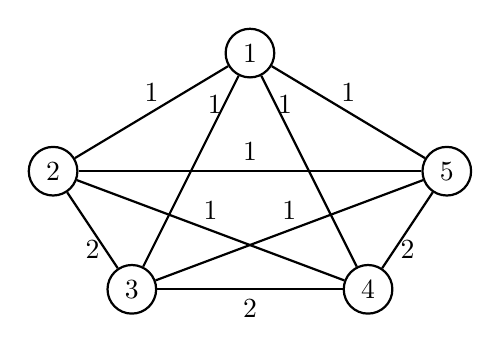
\begin{tikzpicture}[node distance={15mm}, thick, main/.style = {draw, circle}]
% [->,>=stealth,shorten >=1pt,auto,node distance=3cm,
%                         thick,main node/.style={circle,draw,font=\sffamily\Large\bfseries}]
    \node[main] (1) at (1.5,6) {1};
    \node[main] (2) at (-1,4.5) {2};
    \node[main] (3) at (0,3) {3};
    \node[main] (4) at (3,3) {4};
    \node[main] (5) at (4,4.5) {5};

\draw (1) -- (2) node[midway, above] {1};
\draw (1) -- (3) node[near start, above] {1};
\draw (1) -- (4) node[near start, above] {1};
\draw (1) -- (5) node[midway, above] {1};
\draw (2) -- (3) node[midway, below] {2};
\draw (3) -- (4) node[midway, below] {2};
\draw (4) -- (5) node[midway, below] {2};
\draw (4) -- (2) node[midway, above] {1};
\draw (3) -- (5) node[midway, above] {1};
\draw (2) -- (5) node[midway, above] {1};

\end{tikzpicture}

Presupunem ca algoritmul nostru va considera urmatorul $MST$\\

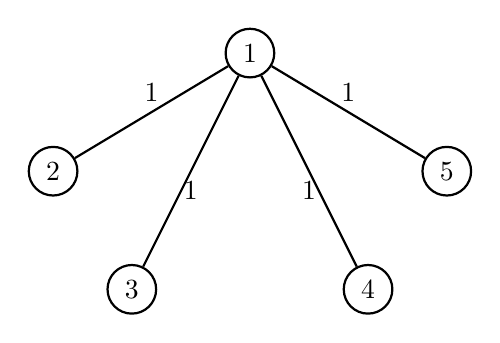
\begin{tikzpicture}[node distance={15mm}, thick, main/.style = {draw, circle}]
% [->,>=stealth,shorten >=1pt,auto,node distance=3cm,
%                         thick,main node/.style={circle,draw,font=\sffamily\Large\bfseries}]
    \node[main] (1) at (1.5,6) {1};
    \node[main] (2) at (-1,4.5) {2};
    \node[main] (3) at (0,3) {3};
    \node[main] (4) at (3,3) {4};
    \node[main] (5) at (4,4.5) {5};

\draw (1) -- (2) node[midway, above] {1};
\draw (1) -- (3) node[midway, below] {1};
\draw (1) -- (4) node[midway, below] {1};
\draw (1) -- (5) node[midway, above] {1};
\end{tikzpicture}

Considerand ca algoritmul din curs nu face nicio optimizare in ordinea in care selecteaza nodurile din $MST$,
algoritmul nostru poate considera ca solutie pentru TSP urmatorul ciclu:\\

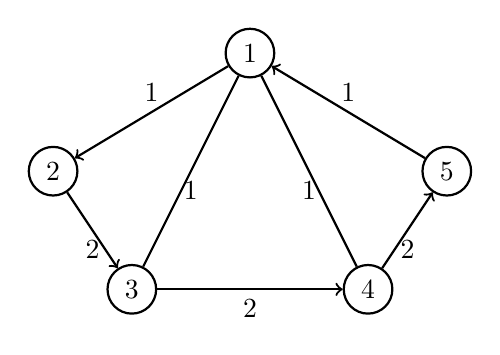
\begin{tikzpicture}[node distance={15mm}, thick, main/.style = {draw, circle}]
    \node[main] (1) at (1.5,6) {1};
    \node[main] (2) at (-1,4.5) {2};
    \node[main] (3) at (0,3) {3};
    \node[main] (4) at (3,3) {4};
    \node[main] (5) at (4,4.5) {5};

\draw[->] (1) -- (2) node[midway, above] {1};
\draw (1) -- (3) node[midway, below] {1};
\draw (1) -- (4) node[midway, below] {1};
\draw[->] (5) -- (1) node[midway, above] {1};
\draw[->] (2) -- (3) node[midway, below] {2};
\draw[->] (3) -- (4) node[midway, below] {2};
\draw[->](4) -- (5) node[midway, below] {2};
\end{tikzpicture}

Deci $ALG=len(1,2,3,4,5,1)=1+2+2+2+1=8$

Dar observam ca in cazul grafului $G$, solutia $OPT$ este:

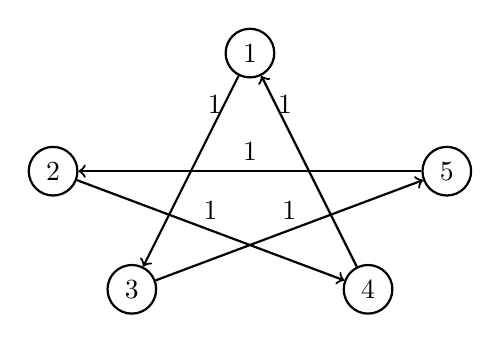
\begin{tikzpicture}[node distance={15mm}, thick, main/.style = {draw, circle}]
    \node[main] (1) at (1.5,6) {1};
    \node[main] (2) at (-1,4.5) {2};
    \node[main] (3) at (0,3) {3};
    \node[main] (4) at (3,3) {4};
    \node[main] (5) at (4,4.5) {5};

\draw[->] (1) -- (3) node[near start, above] {1};
\draw[->] (3) -- (5) node[midway, above] {1};
\draw[->] (5) -- (2) node[midway, above] {1};
\draw[->] (2) -- (4) node[midway, above] {1};
\draw[->] (4) -- (1) node[near end, above] {1};
\end{tikzpicture}

Deci $OPT=len(1,3,5,2,4,1)=1+1+1+1+1=5$\\

Deci avem ca:
\[ALG\leq \frac{3}{2}OPT \Leftrightarrow ALG=8\leq \frac{3}{2}OPT = \frac{3}{2}5 = 7.5 \Leftrightarrow 8\leq 7.5\]

Deci avem ca $ALG> \frac{3}{2}OPT$, adica $ALG$ nu este $\frac{3}{2}$ aproximativ.

\end{document}

